\chapter{پیوست}

\section{جزئیات پیاده‌سازی}
کدهای مربوط به پیاده‌سازی VAE در پوشهٔ `code/` قرار گرفته‌اند. نکات عملی:
\begin{itemize}
    \item فایل آموزشی اصلی: `vae_training.py`
    \item تابع بارگذاری و پیش‌پردازش داده‌ها در `data/` قرار دارد.
    \item برای تولید شکل‌ها و ذخیره‌سازی آن‌ها از توابع تصویرسازی موجود در `utils/visualization.py` استفاده شده است.
\end{itemize}

\section{لیست شکل‌ها (مکان‌نماها)}
شکل‌های مورد نیاز مطابق با `README_FIGURES.md` به صورت مکان‌نما در اینجا آورده شده‌اند. هنگام آماده‌سازی نهایی، فایل‌های PNG معادل را در پوشهٔ `figures/` قرار دهید.

\begin{figure}[H]
    \centering
    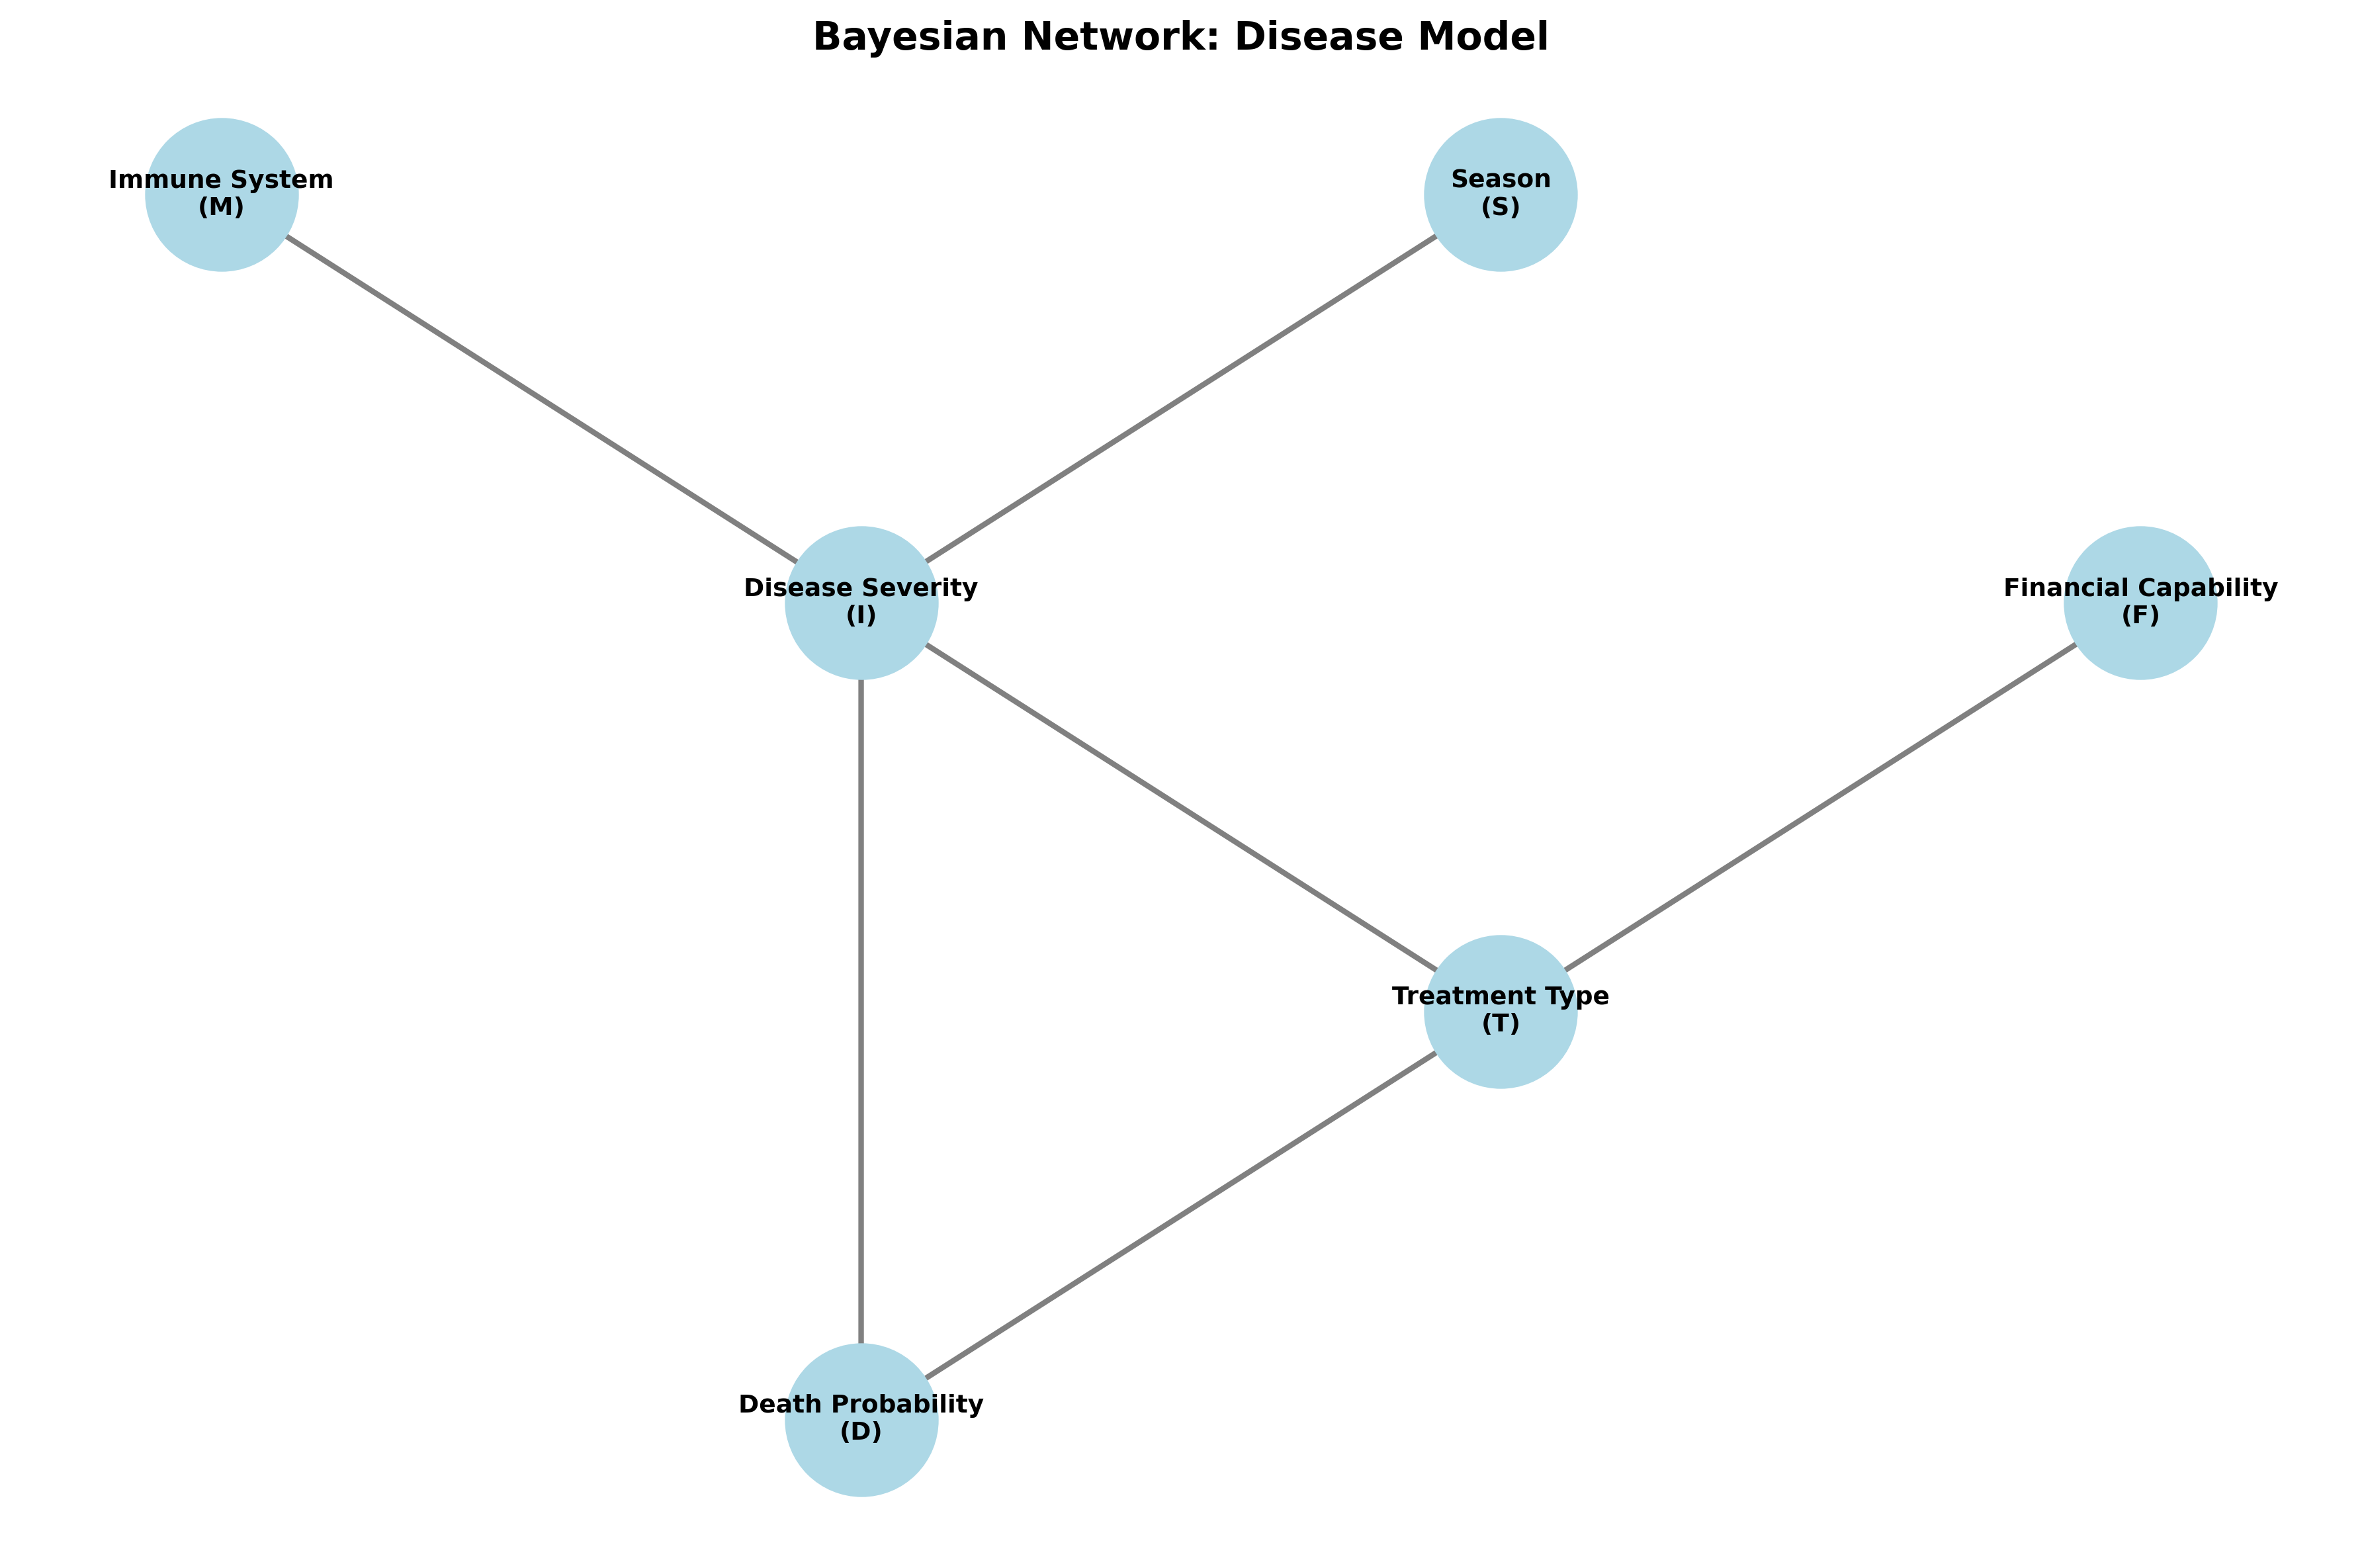
\includegraphics[width=0.7\textwidth]{figures/bayesian_network.png}
    \caption{شبکهٔ بیزی نمونه — مدل سیستم پزشکی}
    \label{fig:bayes_net}
\end{figure}

\begin{figure}[H]
    \centering
    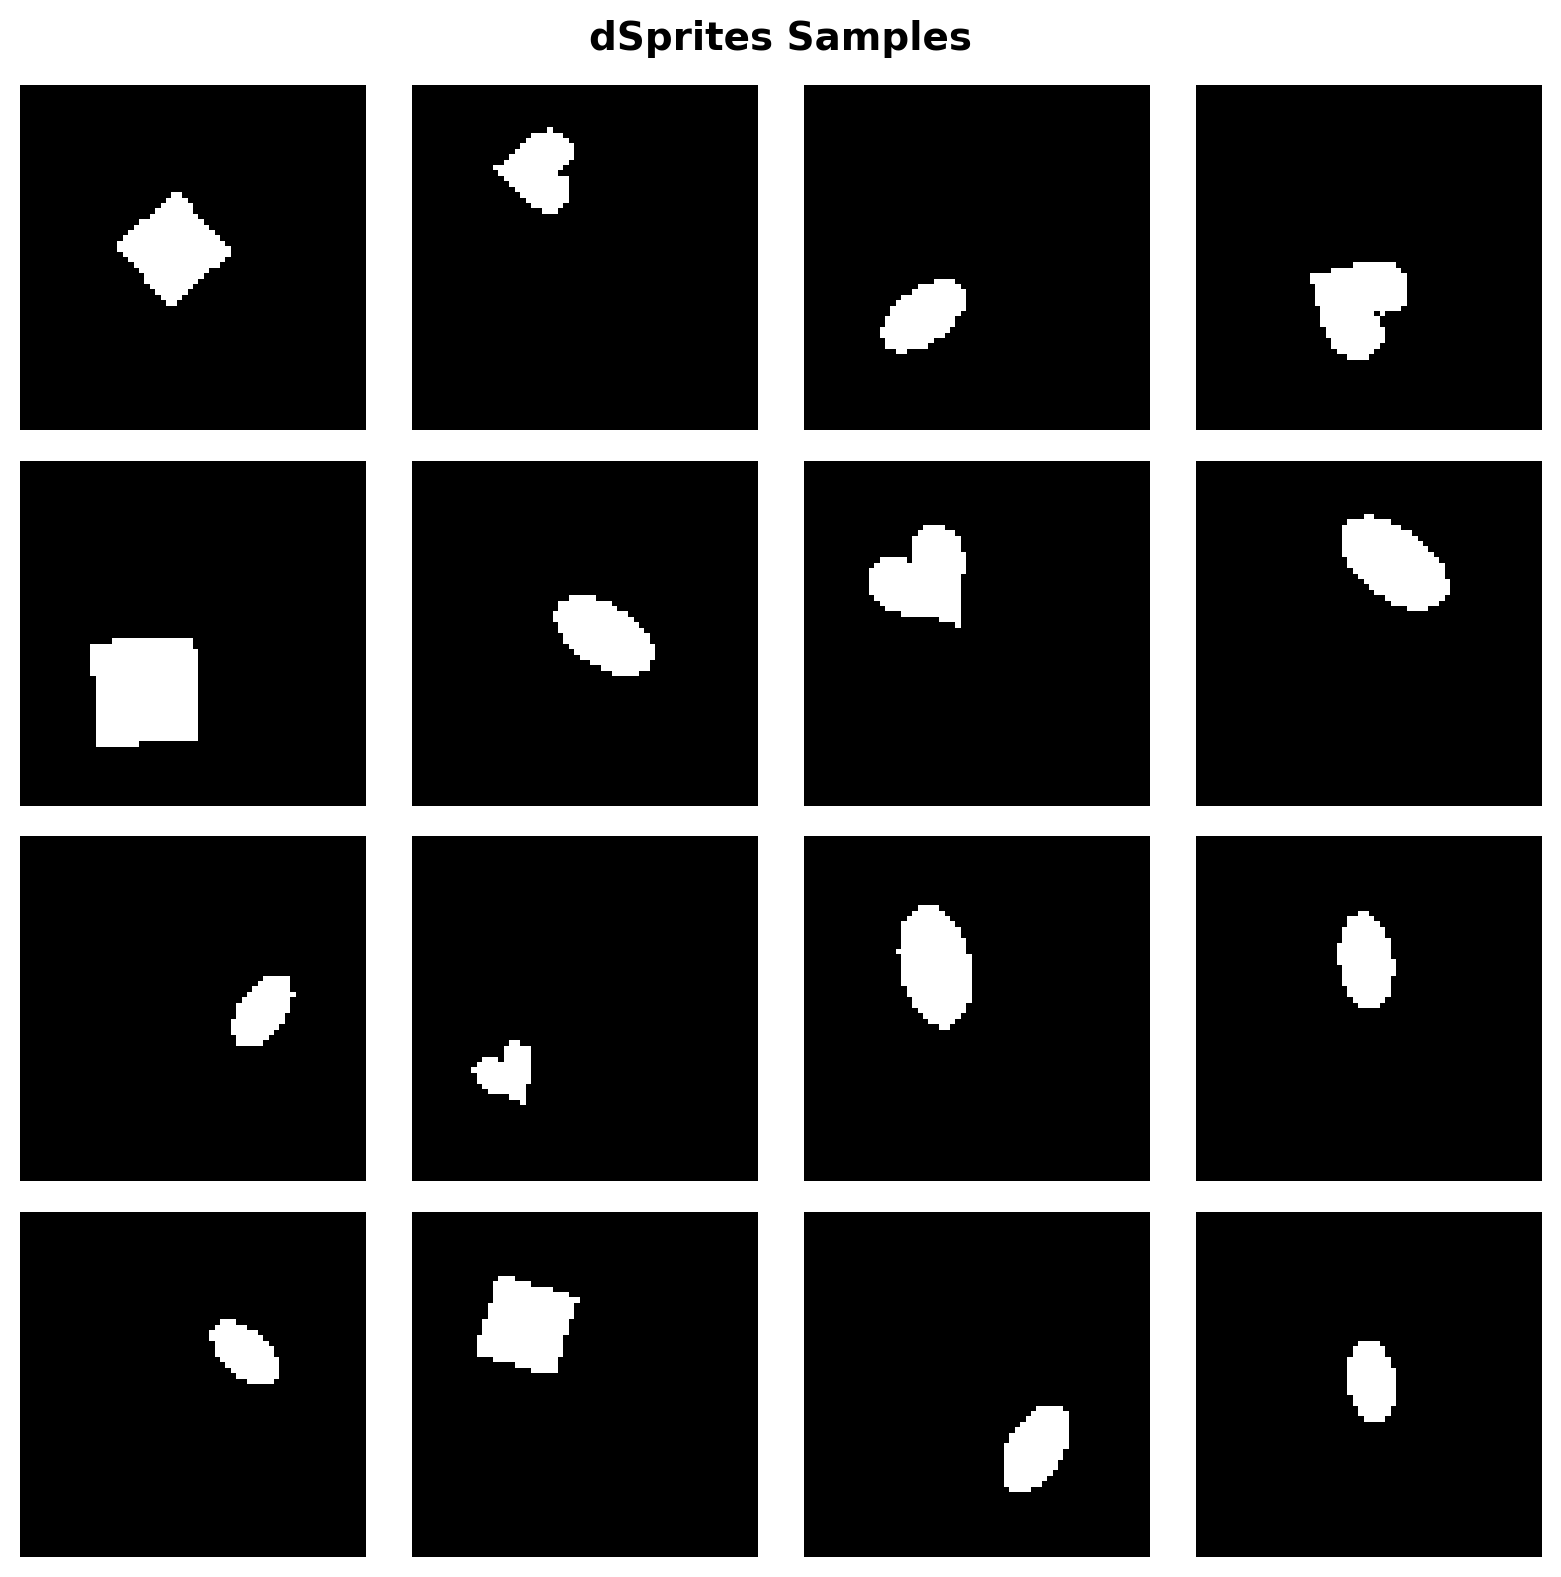
\includegraphics[width=0.7\textwidth]{figures/dsprites_samples.png}
    \caption{نمونه‌هایی از مجموعهٔ dSprites}
    \label{fig:dsprites}
\end{figure}

\begin{figure}[H]
    \centering
    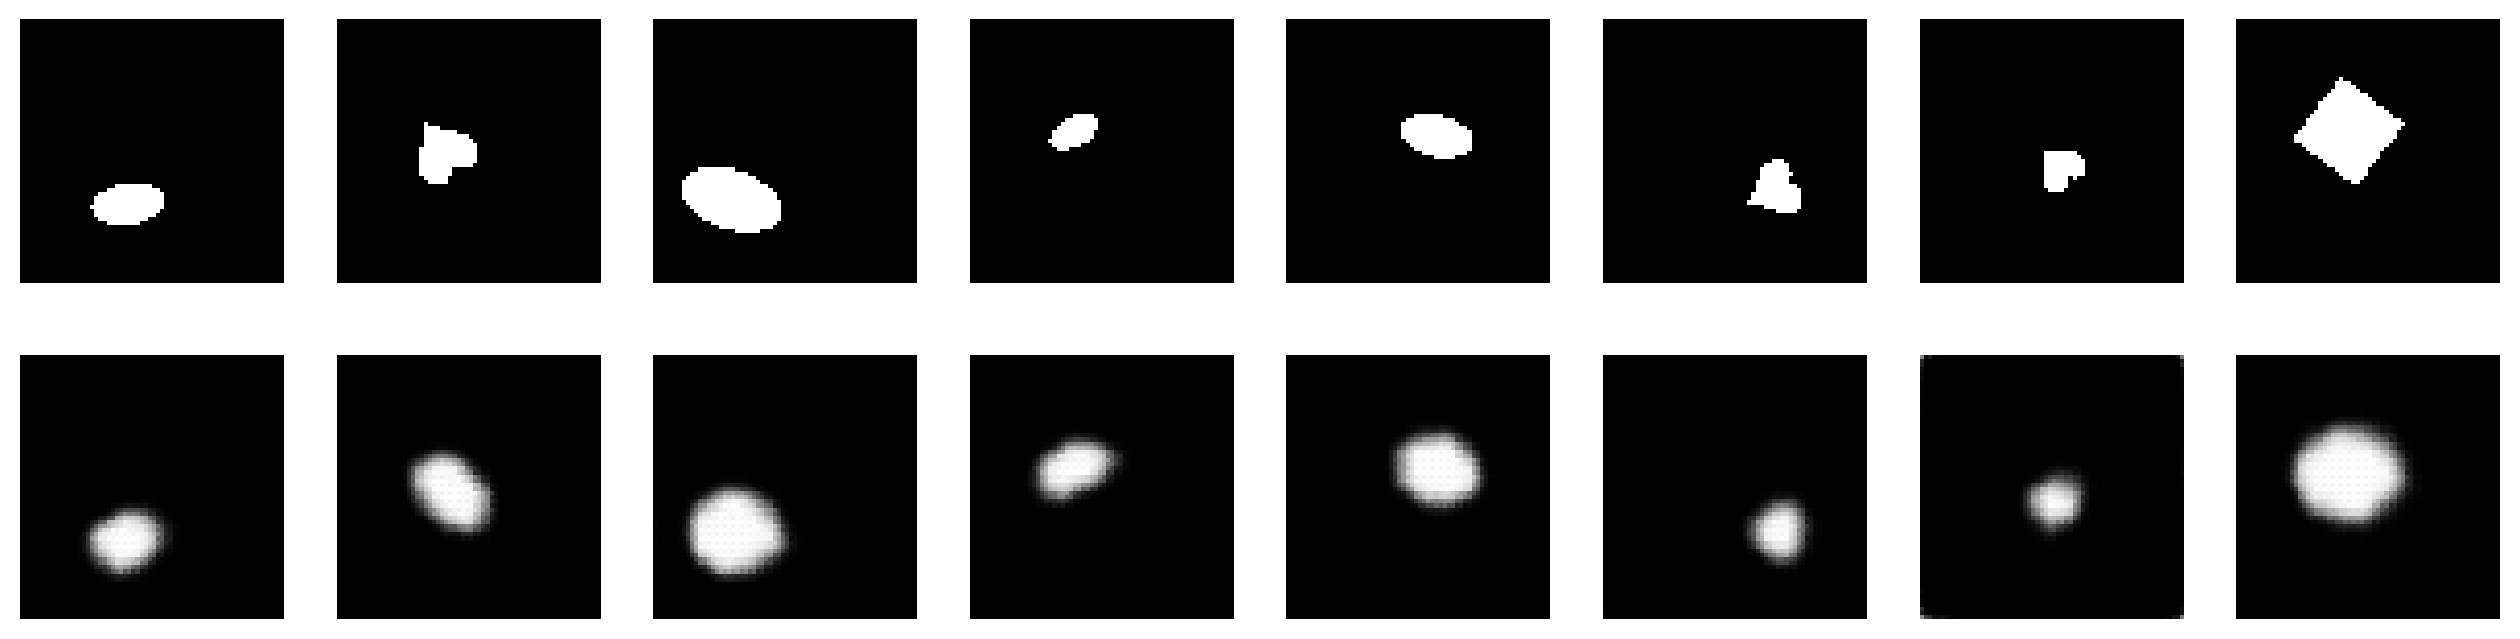
\includegraphics[width=0.7\textwidth]{figures/reconstructions.png}
    \caption{بازسازی‌های مدل (اورجینال در بالا، بازسازی در پایین)}
    \label{fig:recons}
\end{figure}

\section{جداول نمونه}
در صورت نیاز می‌توانید جداول نتایج مقایسه‌ای را به شکل زیر وارد کنید:
\begin{table}[H]
  \centering
  \begin{tabular}{lcc}
    \toprule
    مدل & MSE بازسازی & امتیاز MIG \\
    \midrule
    VAE (\beta=1) & 0.012 & 0.15 \\
    \beta-VAE (\beta=4) & 0.018 & 0.42 \\
    \bottomrule
  \end{tabular}
  \caption{نمونهٔ جدول نتایج}
\end{table}
